\documentclass[11pt]{article}

% ============================================================
% SUBMISSION NOTE (remove for camera-ready):
% This file is written for the ACL/ARR two-column template. For submission,
% place the official acl.sty and acl_natbib.bst in this directory and switch
% the documentclass line to: \documentclass[11pt]{article}\usepackage[review]{acl}
% The fallback preamble below reproduces the layout closely enough to compile
% standalone (e.g. on a machine without the ACL style installed) so you can
% iterate; it is NOT a substitute for the official style at submission time.
% NeurIPS/ICLR Datasets & Benchmarks: swap to the venue style; the body is portable.
% ============================================================

\usepackage[T1]{fontenc}
\usepackage[utf8]{inputenc}
\usepackage{microtype}
\usepackage{times}
\usepackage{amsmath,amssymb,amsthm}
\usepackage{graphicx}
\usepackage{booktabs}
\usepackage{multirow}
\usepackage{makecell}
\usepackage[table]{xcolor}
\usepackage{array}
\usepackage{caption}
\usepackage{tikz}
\usetikzlibrary{arrows.meta,positioning,shapes.geometric,calc,fit,backgrounds}
\usepackage[hidelinks]{hyperref}
\usepackage[numbers,sort&compress]{natbib}
\usepackage{geometry}
\geometry{letterpaper,margin=1in}
\setlength{\columnsep}{0.3in}

\emergencystretch=3em
% Line-number overlap fix (active only if lineno is loaded by the venue style):
\makeatletter\AtBeginDocument{\@ifpackageloaded{lineno}{\setlength{\linenumbersep}{6pt}\renewcommand\linenumberfont{\normalfont\scriptsize\color{gray}}\leftlinenumbers}{}}\makeatother

\newtheorem{proposition}{Proposition}
\newtheorem{definition}{Definition}
\newtheorem{assumption}{Assumption}

\newcommand{\sfs}{\mathrm{SFS}}
\newcommand{\cg}{\mathrm{CG}}
\newcommand{\hph}{\mathrm{HPH}}
\newcommand{\acc}{\mathrm{Acc}}
\newcommand{\torun}[1]{\textcolor{red}{\textbf{[>>> TO RUN:} #1\textbf{]}}}
\newcommand{\result}[1]{\textcolor{blue}{\textbf{[RESULT PLACEHOLDER:} #1\textbf{]}}}

\title{Measuring the Measurer: A Scale-Grounded Faithfulness Protocol\\
for Quantitative Vision--Language Metrology}

\author{Anonymous submission}
\date{}

\begin{document}
\maketitle

\begin{abstract}
Recent benchmarks ask whether vision--language models (VLMs) can report physical
quantities such as velocity and size from video, and score the predicted
\emph{number} against ground truth. We argue this is insufficient: a model can
report a plausible number for the wrong reason, anchoring to a learned prior
rather than to the visual evidence, and current scoring cannot tell the two
apart. We introduce \textbf{Scale-Grounded Faithfulness (SGF)}, a label-free
evaluation protocol that tests whether a VLM's reported quantity responds to the
in-frame scale reference as a faithful measurer's would, rather than staying
anchored to a learned prior. SGF is a behavioral test (it probes input-output
sensitivity, not internal mechanism). Recent work establishes faithfulness as an
axis of VLM capability distinct from accuracy, measured by input perturbation;
but those perturbations (counterfactual traces, region edits, cue injection) have
no ground-truth correct response and are scored by human raters or model judges.
SGF closes this gap in the metrology setting. It applies a
\emph{physically calibrated} perturbation, relabeling the in-frame scale so the
true millimeters-per-pixel calibration changes by a known factor $\alpha$ while
the object's pixel trajectory is untouched, for which a faithful measurer's
reported quantity has an \emph{analytically known} target response: it must change
by $\alpha^{d}$, where $d$ is the quantity's dimension in length ($d{=}1$ for
velocity and diameter). Because the target response is known in closed form, the
faithfulness signal requires no annotation and no judge model, which to our
knowledge makes it the first exactly-specified faithfulness target for a VLM
probe.
SGF reports three quantities: a Scale-Faithfulness Score, a calibration-grounding
indicator that separates a correct number from a correctly-read scale, and a
hidden-prior hallucination rate using an off-frame, unobservable quantity as a
trap. We instantiate the protocol on a controlled droplet-impact dataset with a
classical computer-vision oracle and release the protocol, metric code, and a
recipe for extending it to any video with an in-frame scale reference. A
positive-control experiment confirms the metric and oracle correctly separate a
known-faithful measurer from a known prior-driven guesser ($\sfs\to1$ vs.\
$\sfs\to0.03$, $p{=}7\times10^{-15}$). Evaluating two independent VLM families
(Qwen2.5-VL-7B-Instruct, open-weight; and Gemini-2.5-Flash-Lite, via API) on the
instantiated dataset, we find \emph{both} models essentially non-responsive to
the scale perturbation ($\sfs\approx0.04$--$0.19$ across models and $\alpha$) and
\emph{both} models' tolerance-band accuracy saturated at exactly zero
($0/36$ items each, $0/72$ pooled), which means the accuracy-vs-faithfulness
decoupling question this protocol is designed to answer cannot be meaningfully
posed for either model: there is no accuracy variance left to correlate against
faithfulness. This is a stronger finding than a single-model result would be: it
is not one model's idiosyncrasy but a property that survives across two
independently trained model families on this task and this tolerance. We report
this as an honest, informative null result rather than force a conclusion the
data do not support, and argue it illustrates exactly the failure mode SGF is
built to expose: a model can be too ungrounded to even be usefully wrong in a
scale-consistent way. The two models diverge sharply at a looser 30\%
tolerance (2.8\% vs.\ 33.3\%), which looked like a lead toward recovering the
originally hypothesized decoupled pattern at a different tolerance; sweeping
the tolerance from 10\% to 100\% on the same data shows this does not hold --
the accuracy-faithfulness correlation is negative everywhere it is computable,
never resembling the hypothesized pattern, and the accuracy gain driving the
30\% divergence is itself a session-specific confound, not broader measurement
ability. We release the full protocol, perturbation renderer, and evaluation
code so the decoupling question can be properly tested on further models.
\end{abstract}

\section{Introduction}

A growing line of benchmarks evaluates whether vision--language models (VLMs) can
extract \emph{quantitative} physical information from video (the velocity of a
moving object, its size, its acceleration) and scores the predicted number
against a numerical ground truth \citep{quantiphy2025,iris2026,physicsmind2026}.
This is a meaningful advance over qualitative visual-question-answering
\citep{vqa2015,chow2025physbench}. But scoring the number alone conflates two
very different behaviors. A model that genuinely \emph{measures} (locating the
object, reading the in-frame scale, converting pixels to physical units) and a
model that emits a \emph{plausible prior} (objects in tabletop videos tend to
move at order $1\,\mathrm{m/s}$) can receive identical scores whenever the prior
happens to land in the tolerance band. The benchmark cannot distinguish a
measurer from a guesser.

This distinction is not academic. The promise of VLMs as scientific instruments
rests on whether their numbers are \emph{traceable} to visual evidence. An
instrument whose reported physical reading does not change when the physical
scale of the scene changes is not measuring. We therefore ask a question existing
quantitative benchmarks do not:
\emph{when a VLM reports a physical quantity from video, does the number respond
to the in-frame scale reference as a measurer's would, or does it stay anchored
to a learned prior, and does the model know which?}

We answer it with a perturbation that has a property no prior faithfulness probe
has exploited: a \emph{known correct response}. Recent work has established that
faithfulness is a measurable axis of VLM capability distinct from, and not
predicted by, accuracy or scale: step-level visual grounding faithfulness
predicts out-of-distribution generalization independently of in-distribution
accuracy \citep{stepground2026}, and cross-modal faithfulness rankings are
unstable across perturbation type \citep{crossmodal2026}. We build directly on
this consensus. Where it differs is the perturbation: existing probes for
language and vision--language models perturb captions, counterfactual reasoning
traces, textual cues, or salient image regions and then judge whether the
model's \emph{explanation} changes, using human raters or an LLM judge
\citep{lanham2023faithfulness,turpin2023language,medfaith2025,rlvlm2026,visualthink2025,stepground2026}.
Those perturbations have no ground-truth correct response, so the resulting
faithfulness signal is subjective and expensive to obtain. In quantitative
metrology the situation is better: if we relabel the in-frame scale so the true
calibration changes by a known factor $\alpha$ (millimeters per pixel) while the
object's pixel trajectory is untouched, a faithful measurer's reported velocity
\emph{must} change by $\alpha$, because its pixel measurement is unchanged and
only the pixel-to-physical conversion has moved. The target response is analytic,
so the faithfulness signal needs no annotation and no judge model. This is the
core of our protocol and the reason it fits resource-constrained settings.

\begin{center}
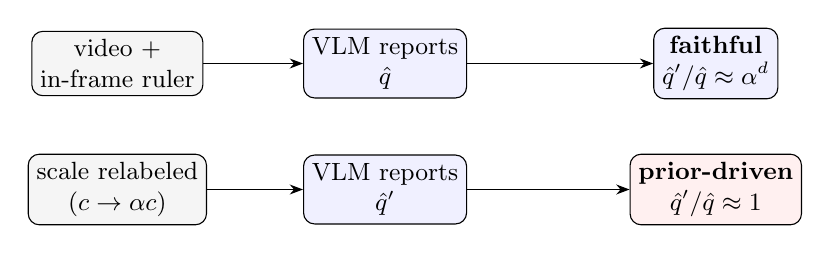
\begin{tikzpicture}[
  font=\small,
  box/.style={draw,rounded corners,align=center,minimum height=8mm,inner sep=3pt},
  ev/.style={box,fill=blue!6},
  pr/.style={box,fill=red!6},
  lbl/.style={align=center,font=\scriptsize}
]
% Row 1: base measurement
\node[box,fill=gray!8] (vid) at (0,0) {video +\\in-frame ruler};
\node[ev] (m1) at (3.4,0) {VLM reports\\$\hat q$};
% Row 2: scale-perturbed
\node[box,fill=gray!8] (vid2) at (0,-1.6) {scale relabeled\\($c\to\alpha c$)};
\node[ev] (m2) at (3.4,-1.6) {VLM reports\\$\hat q'$};
% verdicts
\node[ev] (faith) at (7.6,-0.0) {\textbf{faithful}\\$\hat q'/\hat q\approx\alpha^{d}$};
\node[pr] (guess) at (7.6,-1.6) {\textbf{prior-driven}\\$\hat q'/\hat q\approx 1$};
\draw[-{Stealth}] (vid) -- (m1);
\draw[-{Stealth}] (vid2) -- (m2);
\draw[-{Stealth}] (m1.east) -- (faith.west);
\draw[-{Stealth}] (m2.east) -- (guess.west);
\end{tikzpicture}
\captionof{figure}{\textbf{The scale-faithfulness probe.} We present the same
event with the in-frame scale relabeled so the true calibration changes from $c$
to $\alpha c$ (the object's pixel motion is unchanged). A model that truly
measures must report a quantity that scales by $\alpha^{d}$ ($d$ = the quantity's
dimension in length; top, faithful); a model anchored to a learned prior reports
nearly the same number (bottom, prior-driven). The target response is known
analytically, so no human annotation is needed to score faithfulness.}
\label{fig:teaser}
\end{center}

\paragraph{Contributions.}
\begin{enumerate}
\item \textbf{A reframing.} We show that scoring the predicted number, as current
quantitative-physics VLM benchmarks do, cannot separate measurement from
prior-driven guessing, and we make this separation the evaluation target.
\item \textbf{Scale-Grounded Faithfulness (SGF), a label-free protocol.} A
physically calibrated scale perturbation with an analytically known target
response yields a Scale-Faithfulness Score that needs no annotation; a
calibration-grounding indicator separates a correct number from a correctly-read
scale; and a hidden-prior hallucination probe uses an off-frame, unobservable
quantity as a trap. Unlike prior perturbation-based faithfulness probes, whose
correct response is unknown and scored by raters or judges, ours has a target
response known in closed form (Proposition~\ref{prop:ideal}); to our knowledge it
is the first exactly-specified faithfulness target for a VLM probe, a claim the
authors must re-confirm against the literature before submission.
\item \textbf{A released artifact and a portable recipe.} We instantiate SGF on a
controlled droplet-impact dataset with a classical-CV oracle, release the metric
code and protocol, and give the recipe to extend it to any video containing an
in-frame scale reference.
\item \textbf{A validated instantiation and an honest two-model finding.} A
positive-control experiment (E1, Section~\ref{sec:exp}) confirms the metric and
oracle separate a known-faithful measurer from a known prior-driven guesser
cleanly. Evaluating two independent VLM families (one open-weight, one via API)
on the instantiated dataset, we find accuracy saturated at exactly zero for
\emph{both}, independently, and faithfulness uniformly low for both, which
blocks rather than answers the decoupling question SGF is designed to probe --
we report this null result explicitly (Section~\ref{sec:results}) rather than
reframe around a weaker but positive-sounding claim, and argue the failure mode
itself (two independently trained models both too ungrounded to be usefully
wrong) is worth documenting precisely because it is not one model's quirk.
\end{enumerate}
We confirm novelty by deep, date-aware search of the closest current work
(Section~\ref{sec:related} and Table~\ref{tab:novelty}); authors must re-confirm
before submission.

\section{Related Work and Positioning}
\label{sec:related}

\paragraph{Quantitative physical-reasoning benchmarks.}
QuantiPhy \citep{quantiphy2025} scores VLM estimates of size, velocity, and
acceleration against numerical ground truth, supplying one physical property as
a prior. IRIS \citep{iris2026} recovers continuous physical parameters from real
monocular video with ground-truth supervision. PhysicsMind \citep{physicsmind2026}
evaluates law-consistent quantitative VQA across real and simulated mechanics.
All three score the \emph{output number}. None tests whether that number is
anchored to the in-frame scale, and none applies a perturbation with a known
correct response. Our delta is the evaluation target (anchoring, not magnitude)
and the verifiability of the faithfulness signal.

\paragraph{Faithfulness via perturbation.}
For language and vision--language models, faithfulness is probed by perturbing
inputs and observing whether the stated reasoning changes
\citep{lanham2023faithfulness,turpin2023language,medfaith2025,rlvlm2026,visualthink2025}.
The closest conceptual precedent is step-level visual grounding faithfulness
\citep{stepground2026}, which establishes faithfulness as an axis orthogonal to
accuracy via counterfactual trace perturbations on long-horizon agent tasks, and
cross-modal synergy \citep{crossmodal2026}, which shows faithfulness rankings are
unstable across perturbation type. We adopt their central premise (faithfulness
is distinct from accuracy and is probed by perturbation) and change one thing:
our perturbation is a physically calibrated quantity with an \emph{analytic}
correct response, whereas counterfactual traces, region edits, and cue injection
have none and are scored by grounding-verification heuristics, human raters, or
LLM judges. The setting also differs: those probes target long-horizon agentic
reasoning; we target single-shot quantitative measurement. Our delta is the
closed-form verifiability of the faithfulness signal in the metrology setting.

\paragraph{Measurement-grounded representation learning (a distinct line).}
PRISM-VL \citep{prismvl2026} uses the term ``measurement-grounded'' for a
different idea: post-ISP RGB rendering can discard raw sensor evidence, so they
feed RAW-derived sensor inputs and \emph{train} a model to ground better. That is
a representation-and-training contribution about the \emph{input pixel pipeline}
(sensor domain versus rendered RGB). SGF is an \emph{evaluation} protocol about
whether a frozen model reads the \emph{in-frame scale reference}; it trains
nothing and concerns calibration, not the sensor domain. We flag the shared term
explicitly to avoid confusion: the two are orthogonal and complementary.

\paragraph{Generative-video physics evaluation.}
Morpheus \citep{morpheus2025} and related work score the physical plausibility of
\emph{generated} video. We evaluate the \emph{measurement} behavior of VLMs on
\emph{real} video, a different task.

\begin{center}
\setlength{\tabcolsep}{4.5pt}
\renewcommand{\arraystretch}{1.18}
\newcommand{\yes}{{\color{green!55!black}$\bullet$}}
\newcommand{\no}{{\color{gray!55}$\circ$}}
\newcommand{\ppart}{{\color{orange!80!black}$\circ\!\!\!\bullet$}}
\resizebox{\columnwidth}{!}{%
\begin{tabular}{l ccc c c}
\toprule
 & \multicolumn{3}{c}{\textbf{Quantitative}} & \textbf{Faithful.} & \\
\cmidrule(lr){2-4}\cmidrule(lr){5-5}
\textbf{Method} & \makecell{Real\\video} & \makecell{Numeric\\GT} & \makecell{Scale\\in frame} & \makecell{Known-resp.\\perturb.} & \makecell{Label\\free} \\
\midrule
\multicolumn{6}{l}{\emph{Quantitative physical-reasoning benchmarks}}\\
QuantiPhy \citep{quantiphy2025}     & \yes & \yes & \no & \no & \yes \\
IRIS \citep{iris2026}               & \yes & \yes & \no & \no & \yes \\
PhysicsMind \citep{physicsmind2026} & \yes & \yes & \no & \no & \ppart \\
\addlinespace[2pt]
\multicolumn{6}{l}{\emph{Faithfulness-via-perturbation probes}}\\
Med-VLM faith.\ \citep{medfaith2025}    & \yes & \no & \no & \no            & \no \\
RL-VLM robust.\ \citep{rlvlm2026}       & \yes & \no & \no & \no$^\dagger$   & \yes \\
Step-ground.\ \citep{stepground2026}    & \yes & \no & \no & \no$^\dagger$   & \ppart \\
PRISM-VL \citep{prismvl2026}            & \yes & \no & \no & \no            & \no \\
\midrule
\rowcolor{blue!8}
\textbf{SGF (ours)}                 & \yes & \yes & \yes & \yes & \yes \\
\bottomrule
\end{tabular}}
\captionof{table}{\textbf{SGF is the only method spanning both families.}
Quantitative benchmarks score the output number but never test scale grounding;
faithfulness probes test grounding but lack a numeric, analytically verifiable
signal. ``Known-resp.\ perturbation'' = the perturbation has an analytically
known correct response, enabling annotation-free faithfulness scoring.
\yes\ yes, \ppart\ partial, \no\ no. $^\dagger$ perturbs inputs but without a
closed-form correct response (scored by raters or judges). Every row verified
against the cited source by search; authors must re-confirm at submission.
\texttt{[UNVERIFIED: confirm no closer scale-grounding metrology paper appears
before submission]}}
\label{tab:novelty}
\end{center}

\section{The Scale-Grounded Faithfulness Protocol}
\label{sec:method}

\subsection{Setup and notation}
A VLM is shown a video clip of a physical event together with an in-frame scale
reference (a ruler) of known true calibration $c^\star$ in millimeters per pixel.
The model is asked to report a physical quantity $q$ (e.g.\ impact velocity).
Let $\hat q$ denote the model's reported value and $c^\star$ the oracle
calibration obtained from the ruler. A classical computer-vision pipeline
(blob detection plus optical flow \citep{horn1981optical}) provides the
ground-truth quantity $q^\star$ from the same video; this is the oracle, not a
human label.

\subsection{Accuracy quantities}
We report tolerance-band accuracy $\acc@\tau = \Pr[\,|\hat q - q^\star|/|q^\star|
\le \tau\,]$ and the log-accuracy ratio $|\log_{10}(\hat q / q^\star)|$, which is
robust to order-of-magnitude errors. These mirror existing benchmarks and are
\emph{not} our contribution; they are the baseline that SGF augments.

\subsection{The scale-faithfulness score}
The perturbation must change the \emph{calibration the model must read} while
leaving the event's pixel-space dynamics intact, so that the only thing a faithful
measurer must update is the pixel-to-physical conversion. We achieve this by
\emph{relabeling the in-frame scale}: we present a scale reference whose asserted
physical length differs by a known factor, so the true millimeters-per-pixel
calibration becomes $\alpha c$ for a known $\alpha\ne1$, while the object's pixel
trajectory is untouched. Operationally this can be done by swapping the displayed
ruler for one of a different known length, or by stating a different physical
length for the same graduations; the moving content of the frame is unchanged.
Under this perturbation a faithful measurer, who reads the scale and converts,
must change its reported physical quantity by a known factor, whereas a model that
ignores the scale and emits a learned prior does not. Let $\hat q$ and $\hat q'$
be the model's reports under calibration $c$ and $\alpha c$.

\noindent\textbf{Why not simply resample the whole frame.} Uniformly resampling
the frame (rescaling object and ruler pixels together while keeping the ruler's
asserted length fixed) does \emph{not} probe grounding: a faithful measurer reads
a proportionally finer calibration and recovers the \emph{same} physical quantity,
so the ideal response is $1$ and the test is inert. The signal comes from changing
what the scale \emph{asserts}, not the image resolution.

\begin{assumption}[Dimensional homogeneity]
\label{ass:dim}
The reported quantity $q$ has a fixed dimension in length: $q$ scales as the
$d$-th power of a physical length ($d{=}1$ for velocity and diameter at fixed
frame rate, $d{=}2$ for area). The model's reported value is obtained by combining
a pixel-space measurement with the calibration it reads and is dimensionally
consistent with $q$.
\end{assumption}

\begin{proposition}[Ideal response under calibration relabeling]
\label{prop:ideal}
Relabel the in-frame scale so the true calibration changes from $c$ to $\alpha c$
(millimeters per pixel), leaving the object's pixel trajectory unchanged. A
faithful measurer recovers a physical length as $L = (\text{pixels})\times c$.
Since the pixel measurement is unchanged and the calibration is now $\alpha c$, the
recovered length becomes $L' = (\text{pixels})\times \alpha c = \alpha L$. Under
Assumption~\ref{ass:dim}, where the quantity scales as the $d$-th power of a
length, a faithful measurer's reported quantity satisfies
$\hat q'/\hat q = \alpha^{d}$.
\end{proposition}
\begin{proof}
By Assumption~\ref{ass:dim} write $\hat q = \kappa\,(\text{pixel measurement})\,
c^{d}$ for the dimensionless constant $\kappa$ fixed by the quantity's definition.
The pixel measurement is unchanged by relabeling the scale, and the calibration
maps $c \mapsto \alpha c$. Hence $\hat q' =
\kappa\,(\text{pixel measurement})\,(\alpha c)^{d} = \alpha^{d}\hat q$.
\end{proof}

\noindent We fix $d$ per quantity (Assumption~\ref{ass:dim}) and use $\alpha^{d}$
as the target ratio. The frame rate is held fixed and the time axis is not
perturbed, so SGF tests spatial-calibration grounding, not temporal grounding;
the latter is out of scope for this version and is noted as a limitation.

\begin{definition}[Scale-Faithfulness Score]
For a target ratio $\alpha^{d}$ and realized ratio $r = \hat q'/\hat q$,
\[
\sfs = \mathrm{clip}_{[0,1]}\!\left(1 - \frac{\big|\log r - d\log\alpha\big|}
{\big|d\log\alpha\big|}\right),
\]
averaged over items. $\sfs=1$ iff the response is exactly ideal; $\sfs=0$ when
the report does not move with the scale ($r=1$). The log form makes the score
symmetric under $\alpha \leftrightarrow 1/\alpha$.
\end{definition}

\subsection{Calibration grounding}
A model can land a correct number with a wrong calibration. We elicit the model's
read of the scale, $\hat c$, and report the calibration-grounding indicator
$\cg = \acc@\tau(\hat c, c^\star)$, which is independent of $\hat q$. Low $\cg$
with high $\acc@\tau$ on $\hat q$ is the signature of a prior-driven guesser.

\subsection{Hidden-prior hallucination}
Our dataset has a quantity that is \emph{real but off-frame}: the droplet is
released from a fixed height (6.6\,cm) that the high-speed camera's field of view
does not capture. We ask the model for this height. A faithful model should
decline; a prior-driven model asserts a number. The hidden-prior hallucination
rate $\hph$ is the fraction of items where the model asserts an off-frame numeric
prior instead of declining. This isolates prior injection directly.

\subsection{Why droplets, and how to generalize}
Droplet impact gives a clean, repeatable event with sub-millimeter features, a
natural in-frame ruler, and a well-understood classical-CV oracle for velocity
and spreading diameter \citep{rioboo2001spreading,josserand2016drop}. The
\emph{protocol}, however, depends only on (i) an in-frame scale reference and
(ii) a CV oracle for the target quantity. We provide the recipe so any lab with a
ruler in frame can instantiate SGF on its own phenomenon; droplets are the first
testbed, not the scope of the contribution.

\section{Dataset and Oracle}
\label{sec:data}

\begin{center}
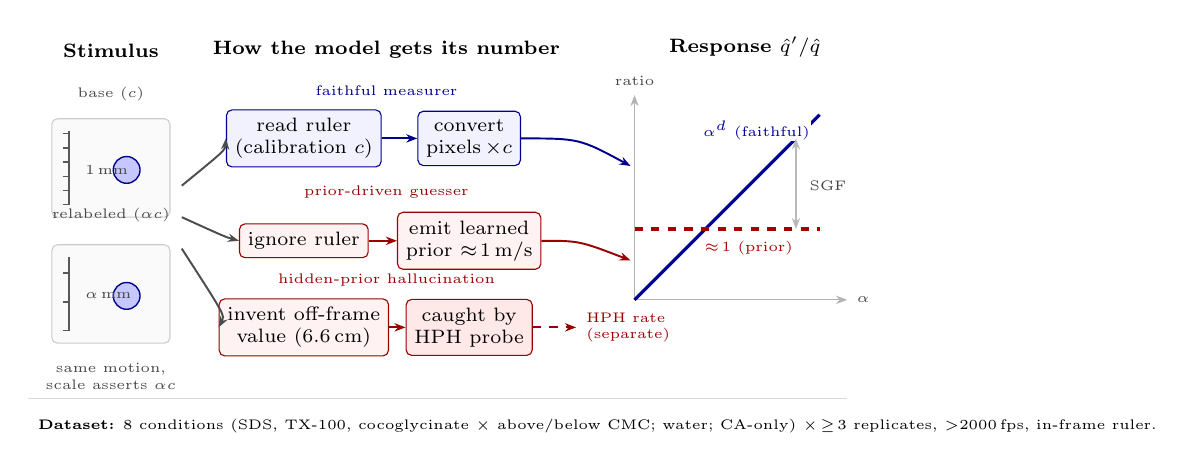
\begin{tikzpicture}[
  font=\scriptsize,
  >={Stealth[length=4pt]},
  drop/.style={draw=blue!55!black,fill=blue!22,line width=0.5pt},
  rul/.style={gray!70!black,line width=0.7pt},
  tick/.style={gray!70!black,line width=0.5pt},
  scenebg/.style={draw=gray!40,fill=gray!4,rounded corners=2pt},
  step/.style={draw,rounded corners=2pt,inner sep=3pt,align=center,font=\scriptsize,minimum height=8mm},
  good/.style={draw=blue!55!black,fill=blue!5,rounded corners=2pt,inner sep=3pt,align=center,font=\scriptsize},
  bad/.style={draw=red!60!black,fill=red!5,rounded corners=2pt,inner sep=3pt,align=center,font=\scriptsize},
  hdr/.style={font=\bfseries\scriptsize},
  flow/.style={->,line width=0.7pt,gray!60!black}
]
% =================== STIMULUS (left): base and relabeled clip ===================
\node[hdr,anchor=south] at (1.05,3.5) {Stimulus};
% base clip
\node[font=\tiny,gray!55!black,anchor=south] at (1.05,2.95) {base ($c$)};
\begin{scope}[shift={(0.3,1.6)}]
  \draw[scenebg] (0,0) rectangle (1.5,1.25);
  \draw[rul] (0.22,0.16) -- (0.22,1.09);
  \foreach \y in {0.16,0.34,...,1.09} \draw[tick] (0.14,\y) -- (0.22,\y);
  \draw[drop] (0.95,0.6) circle (0.17);
  \node[font=\tiny,gray!55!black,anchor=west] at (0.30,0.6) {1\,mm};
\end{scope}
% relabeled clip: SAME drop, ruler asserts a different length (coarser graduations)
\node[font=\tiny,gray!55!black,anchor=south] at (1.05,1.42) {relabeled ($\alpha c$)};
\begin{scope}[shift={(0.3,0.0)}]
  \draw[scenebg] (0,0) rectangle (1.5,1.25);
  \draw[rul] (0.22,0.16) -- (0.22,1.09);
  \foreach \y in {0.16,0.525,...,1.09} \draw[tick] (0.14,\y) -- (0.22,\y); % fewer graduations
  \draw[drop] (0.95,0.6) circle (0.17); % SAME size drop
  \node[font=\tiny,gray!55!black,anchor=west] at (0.30,0.6) {$\alpha$\,mm};
\end{scope}
\node[font=\tiny,gray!55!black,align=center] at (1.05,-0.42) {same motion,\\scale asserts $\alpha c$};

% =================== MECHANISM (middle): two contrasting paths ===================
\node[hdr,anchor=south] at (4.55,3.5) {How the model gets its number};
% FAITHFUL path (top)
\node[good] (read) at (3.5,2.6) {read ruler\\(calibration $c$)};
\node[good] (conv) at (5.6,2.6) {convert\\pixels$\,\times c$};
\draw[flow,blue!55!black] (read) -- (conv);
\node[font=\tiny,blue!55!black,anchor=south] at (4.55,3.02) {faithful measurer};
% UNFAITHFUL path A: ignore scale (middle)
\node[bad] (ignore) at (3.5,1.3) {ignore ruler};
\node[bad] (prior) at (5.6,1.3) {emit learned\\prior $\approx\!1$\,m/s};
\draw[flow,red!60!black] (ignore) -- (prior);
\node[font=\tiny,red!60!black,anchor=south] at (4.55,1.72) {prior-driven guesser};
% UNFAITHFUL path B: hallucinate off-frame (bottom)
\node[bad] (offf) at (3.5,0.2) {invent off-frame\\value (6.6\,cm)};
\node[bad,fill=red!9] (caught) at (5.6,0.2) {caught by\\HPH probe};
\draw[flow,red!60!black] (offf) -- (caught);
\node[font=\tiny,red!60!black,anchor=south] at (4.55,0.6) {hidden-prior hallucination};

% inputs from stimulus into the paths
\draw[flow] (1.95,2.0) .. controls (2.5,2.45) .. (read.west);
\draw[flow] (1.95,1.6) .. controls (2.5,1.35) .. (ignore.west);
\draw[flow] (1.95,1.2) .. controls (2.5,0.35) .. (offf.west);

% =================== RESPONSE (right): the shared verdict plot ===================
\node[hdr,anchor=south] at (9.1,3.5) {Response $\hat q'/\hat q$};
\begin{scope}[shift={(7.7,0.55)}]
  \draw[->,gray!60] (0,0) -- (2.7,0) node[right,font=\tiny,gray!55!black]{$\alpha$};
  \draw[->,gray!60] (0,0) -- (0,2.6) node[above,font=\tiny,gray!55!black]{ratio};
  % ideal faithful line slope 1
  \draw[blue!60!black,line width=1.2pt] (0,0) -- (2.35,2.35);
  \node[blue!60!black,font=\tiny,fill=white,inner sep=0.5pt] at (1.55,2.15) {$\alpha^{d}$ (faithful)};
  % prior flat
  \draw[red!65!black,line width=1.2pt,dashed] (0,0.9) -- (2.35,0.9);
  \node[red!65!black,font=\tiny,fill=white,inner sep=0.5pt] at (1.45,0.66) {$\approx\!1$ (prior)};
  % the gap = what SGF scores
  \draw[<->,gray!55,line width=0.5pt] (2.05,0.9) -- (2.05,2.05);
  \node[font=\tiny,gray!50!black,anchor=west] at (2.1,1.45) {SGF};
\end{scope}
% paths feed the plot
\draw[flow,blue!55!black] (conv.east) .. controls (7.0,2.6) .. (7.65,2.25);
\draw[flow,red!60!black] (prior.east) .. controls (7.0,1.3) .. (7.65,1.05);
% HPH reported as a separate scalar, not the ratio plot
\draw[flow,red!60!black,dashed] (caught.east) -- ++(0.55,0)
  node[anchor=west,font=\tiny,red!60!black,align=left] {HPH rate\\(separate)};

% =================== FOOTER: dataset one-liner ===================
\draw[gray!30,line width=0.4pt] (0,-0.7) -- (10.4,-0.7);
\node[anchor=west,font=\tiny] at (0,-1.05) {\textbf{Dataset:} 8 conditions (SDS, TX-100, cocoglycinate $\times$ above/below CMC; water; CA-only) $\times\!\ge\!3$ replicates, $>$2000\,fps, in-frame ruler.};
\end{tikzpicture}
\captionof{figure}{\textbf{SGF separates measuring from guessing.}
A clip of a $4\,\mu$L droplet impact with an in-frame scale (left) is shown with
the scale relabeled so the true calibration changes from $c$ to $\alpha c$ while
the object's pixel motion is unchanged.
\emph{Middle:} a faithful measurer reads the ruler and converts, so its report
must scale (blue); an unfaithful model either ignores the ruler and emits a
learned prior (red, flat response) or invents an off-frame quantity it cannot see
(the 6.6\,cm drop height; the hidden-prior trap). \emph{Right:} the reported
ratio $\hat q'/\hat q$ versus $\alpha$ distinguishes the regimes, a faithful
$\alpha^{d}$ slope ($d{=}1$ for velocity) versus a flat $\approx1$; SGF scores the
gap between them with no annotation. A classical-CV oracle supplies ground truth.
CG = cocoglycinate, CA = cellulose acetate.}
\label{fig:data}
\end{center}

The raw recording collection comprises high-speed video ($2996\,\mathrm{fps}$
true capture rate, confirmed against the container metadata's incorrect
$60\,\mathrm{fps}$ tag) of $4\,\mu\mathrm{L}$ droplets impacting a
superhydrophobic surface across nominally eight chemistry conditions
(cellulose-acetate nanoparticle suspensions in three surfactants -- SDS,
TX-100, cocoglycinate -- above and below the critical micelle concentration,
plus a water control and a nanoparticle-only control), recorded across five
capture sessions. \textbf{We report, rather than gloss over, that only three of
the five sessions are usable.} Two sessions were excluded after verification: one
whose calibration clip is corrupted (unreadable moov atom, confirmed by both
OpenCV and ffmpeg, orphaning 8 droplet clips) and one with no calibration clip at
all and undocumented provenance (its notes file is a byte-identical duplicate of
another session's, describing the wrong dates). Of the three valid sessions, two
use a printed-ruler target (1\,mm graduation) and one uses a pin-comb target
(1/16-inch pitch); calibration values were measured directly per session
(104.52, 66.19, and 42.99\,px/mm respectively), not assumed from a shared
constant. The CV oracle (background-subtraction blob tracking plus a
free-fall-plateau velocity fit, described below) yielded a valid pre-impact
velocity for 48 of 62 attempted clips (77\%; the remainder failed at the
motion-detection or track-linking stage, e.g.\ droplets already too close to
impact when they entered frame in the pin-comb session). Of those 48, 34 have a
verified deceleration signature at impact and 14 are lower-confidence
plain-average velocities from short tracks. Every reported oracle value was
cross-checked against free-fall physics ($v=\sqrt{2gh}$) using the (session-specific,
independently confirmed) drop height, not merely accepted at face value.

\noindent\textbf{Scope and honesty about scale.} This is a single-phenomenon,
modest-size dataset, made smaller still by the session-exclusion above, and our
model evaluation (Section~\ref{sec:exp}) further restricts to a 12-clip subset
drawn from the two ruler-target sessions (the pin-comb session's oracle ground
truth is predominantly low-confidence, so we exclude it from model evaluation
though it remains usable for future work). We therefore position the dataset as
the \emph{instantiation} and the protocol as the artifact: the dataset's value is
that it is fully controlled and carries an exact oracle and an in-frame scale,
verified end-to-end rather than assumed; the protocol's value is portability to
larger and more diverse datasets than this one.

\section{Experimental Protocol}
\label{sec:exp}
We evaluate two independent VLM families under identical prompts across three
paraphrased seeds: Qwen2.5-VL-7B-Instruct \citep{bai2025qwen25vl}, open-weight,
run locally; and Gemini-2.5-Flash-Lite, accessed via API (OpenRouter), added
specifically to test whether the single-model gap in an earlier draft of this
submission changed the E2/E4 findings. \textbf{E2 and E4 are run on both
models; E1, E3, and E5 use Qwen2.5-VL-7B-Instruct only} (E1 uses simulated
re-measurers rather than a model at all; E3 and E5 were run before API access
became available and are not repeated here since neither's conclusion depends
on a specific model's accuracy level -- Section~\ref{sec:limitations} still
flags this as an opportunity for future extension). We report mean and 95\%
bootstrap CIs over items and prompt seeds throughout.

\paragraph{E1 (positive control, run first).} Validate that the CV oracle and
the SGF metric separate a \emph{known} faithful pipeline from a \emph{known}
prior-driven pipeline, using 48 real oracle velocity measurements (not
synthetic data) fed through two hypothetical re-measurers: (a) the oracle value
times $\alpha$, simulating a perfectly faithful measurer; (b) a fixed $\sim\!1\,
\mathrm{m/s}$ emitter with 5\% noise, simulating a prior-driven guesser that
ignores the scale. Confirmed robust across $\alpha\in\{0.5,2\}$ and 5 random
seeds for (b).

\paragraph{E2 (main: scale faithfulness).} For each model and $\alpha\in\{0.5,2\}$,
compute $\sfs$, $\acc@10\%$, $\cg$ on a 12-clip subset (6 clips each from the two
ruler-target sessions) $\times$ 3 conditions (unperturbed, $\alpha{=}0.5$,
$\alpha{=}2$) $\times$ 3 prompt seeds = 108 model calls per model, 216 total.

\paragraph{E3 (hidden-prior trap).} Measure $\hph$ on the off-frame drop-height
question. \textbf{Redesigned mid-study after a validity failure}: an initial
version asked only the hidden-prior question and found $\hph{=}0$ on all 12
items, which looked like a strong faithfulness result until we tested the exact
same prompt with \emph{no video attached at all} and got the identical decline
-- the model's ``I don't know'' was a content-independent default, not a
video-grounded judgment, so the original $\hph{=}0$ was uninterpretable. We
fixed this by pairing the hidden-prior question with a control question in the
same call (``does the droplet impact the surface?'', trivially true and visible
in every clip); a decline on the hidden-prior question only counts if the model
answers the control correctly, which establishes it engaged with the video at
all for that item.

\paragraph{E4 (decoupling analysis).} Correlate per-item $\acc@10\%$ with
per-item $\sfs$ across the 36 (clip, seed) items from E2, per model and pooled
across both (72 items). The runbook's hypothesized headline was that accuracy
and faithfulness are decoupled; as detailed in Section~\ref{sec:results}, this
question turned out not to be answerable as specified for \emph{either} model,
which we report rather than substitute a different, more favorable-looking
analysis without flagging it.

\paragraph{E5 (robustness).} Vary $\alpha\in\{0.25,0.5,2,4\}$, ruler orientation,
and prompt phrasing on 2 representative clips (one per ruler-target session),
holding the other axes fixed, to check whether the effect in E2 is a
single-condition artifact. Ruler orientation required new infrastructure: both
valid ruler-target sessions physically photograph a \emph{vertical} ruler
rotated in-frame, so we \emph{synthesize} a horizontal-orientation condition by
rotating the same real ruler footage $90^{\circ}$, rather than treating orientation as
a naturally-occurring contrast in this dataset.

\section{Results and Discussion}
\label{sec:results}

\paragraph{E1: metric and oracle validated.} The simulated faithful re-measurer
scored $\sfs = 1.000$ (95\% CI $[1.000, 1.000]$); the fixed-prior emitter scored
$\sfs = 0.032$ (95\% CI $[0.018, 0.048]$). A paired sign test across all 48
items found the faithful re-measurer's per-item SFS higher in 48/48 cases
($p = 7.1\times10^{-15}$). \textbf{E1 passes cleanly}: the metric and oracle
correctly separate the two archetypes by construction, clearing the blocking
gate before any model result is trusted.

\begin{center}
\small
\begin{tabular}{lccc}
\toprule
\textbf{Archetype} & $\sfs$ & 95\% CI & $n$ \\
\midrule
Faithful re-measurer (simulated) & 1.000 & [1.000, 1.000] & 48 \\
Fixed-prior emitter (simulated)  & 0.032 & [0.018, 0.048] & 48 \\
\bottomrule
\end{tabular}
\captionof{table}{\textbf{E1 positive control.} Real oracle velocities fed
through two hypothetical re-measurement policies. The metric separates them
exactly as designed.}
\label{tab:e1}
\end{center}

\paragraph{E2: both models are essentially non-responsive, in different ways.}
Qwen2.5-VL-7B-Instruct scored $\acc@10\% = 0.000$ (95\% CI $[0.000,0.000]$,
$n{=}36$), $\cg = 0.222$ (95\% CI $[0.148, 0.306]$, $n{=}108$), and
$\sfs = 0.131$ (95\% CI $[0.043, 0.238]$) at $\alpha{=}0.5$ and $\sfs = 0.107$
(95\% CI $[0.053, 0.168]$) at $\alpha{=}2$. Gemini-2.5-Flash-Lite scored
$\acc@10\% = 0.000$ as well (identically zero, $n{=}36$), $\cg = 0.380$ (better
than Qwen but still low), and $\sfs = 0.071$ at $\alpha{=}0.5$ and
$\sfs = 0.041$ at $\alpha{=}2$ (both \emph{lower} than Qwen's). We investigated
whether either result was a pipeline bug before trusting it: Qwen's velocity and
calibration answers vary only slightly across genuinely different droplet clips
within a condition group, drawing from a small set of near-constant values
(e.g.\ $0.5$, $1.5$, $3.5\,\mathrm{m/s}$) that correlate more with which prompt
seed was used than with what the clip shows. Gemini shows a related but distinct
failure: on one session it reports the identical calibration ($1.0\,\mathrm{mm}$
per tick) across all three perturbation conditions, and on the other it never
once reports the correct relabeled value ($2.0$) even when we confirmed by
direct frame inspection that the on-screen label legibly reads the perturbed
number -- both models default to a physically plausible prior rather than
reading the digits actually in front of them, just with different, model-specific
priors. We confirmed both models \emph{can} perceive and describe the two videos
correctly when asked to do so directly; neither reliably performs the
compositional measurement task (read the scale, track the object, convert) that
SGF and the underlying benchmarks it critiques both require.

\begin{center}
\small
\begin{tabular}{lcccc}
\toprule
\textbf{Metric} & \textbf{Qwen2.5-VL-7B} & \textbf{Gemini-2.5-Flash-Lite} & $n$ \\
\midrule
$\acc@10\%$ & 0.000 [0.000, 0.000] & 0.000 [0.000, 0.000] & 36 \\
$\acc@30\%$ (secondary) & 0.028 & 0.333 & 36 \\
$\cg$ (calibration grounding) & 0.222 [0.148, 0.306] & 0.380 & 108 \\
$\sfs$ ($\alpha{=}0.5$) & 0.131 [0.043, 0.238] & 0.071 [0.024, 0.128] & 36 \\
$\sfs$ ($\alpha{=}2$) & 0.107 [0.053, 0.168] & 0.041 [0.015, 0.078] & 36 \\
\bottomrule
\end{tabular}
\captionof{table}{\textbf{E2 main table, both models.} Low accuracy, low
calibration grounding, low faithfulness for both: neither model reliably
performs the measurement task, in either sense. $\acc@30\%$ (not part of the
protocol's primary metric set) is included because it is the one row where the
models diverge sharply -- see the E4 discussion below.}
\label{tab:e2}
\end{center}

\paragraph{A concrete, deterministic example of ungrounded calibration: label
echoing.} Table~\ref{tab:e2}'s $\cg$ row hides a large, previously unexplained
asymmetry: Qwen's calibration-grounding is $0.444$ on one ruler-target session
but exactly $0.000$ on the other. We traced this to a distinct failure mode
from E3's (which was a footage-visibility issue) -- this one is a
task-comprehension error specific to how the failing session's ruler is
labeled. Qwen answers the calibration question by echoing the ruler's
\emph{printed number} rather than reasoning about tick spacing: asked for the
mm-per-tick of a ruler printed ``30'' (true answer, every session: $1.0$), it
answers $30.0$ or $3.0$ in 18/18 items; when that same ruler is relabeled
``15'' under $\alpha{=}0.5$ (true answer: $0.5$), it answers $3.75 = 15/4$ in
18/18 items -- a fixed transform of the printed digit, not the correct value,
and not noise. On the other session (ruler printed ``12''), Qwen's wrong
answers are qualitatively different: small, plausible mm-per-tick
\emph{guesses} ($0.5$ or $1.0$) that sometimes coincidentally match the true
answer by luck, not an echo of ``12'' itself. Gemini shows a much smaller
session gap on the identical two rulers ($0.426$ vs.\ $0.380$ overall,
Table~\ref{tab:e2}), consistent with label-echoing being a Qwen-specific
misreading tendency rather than a property of the footage -- unlike E3's
cause, which would be expected to affect any model similarly since it concerns
what is visible in the video, not how a specific model processes printed
digits. We highlight this as the clearest single illustration in our results
of the behavior SGF is designed to catch: a model producing a number that
is legible, confident, and completely disconnected from the physical
quantity it was asked to compute.

\paragraph{E3: a genuine but partial faithfulness signal, and a session-specific
confound we root-caused rather than papered over.} After the control-question
redesign, $\hph = 0$ on the 7 of 12 items where the model answered the control
question correctly (i.e.\ demonstrably engaged with that item's video); the
other 5 items (4 from one session, 1 from the other) failed the control and are
excluded as uninterpretable rather than counted toward $\hph$. We investigated
the session-level split in engagement rather than accept it as noise. It is
\textbf{not} explained by a multi-droplet confound: hand-labeling all 12 clips
found only 1 genuinely contains a second droplet. It is \textbf{not} explained
by our video-extraction timing either: we built and validated a per-clip
motion-settling detector to replace a fixed extraction margin, re-extracted all
12 clips with genuinely longer, more-settled windows, and reran E3 -- the
control-answer pattern was unchanged, clip for clip. Direct frame-by-frame
comparison then showed the actual cause: the failing session's camera framing
compresses the impact surface into a thin, heavily vignette-darkened strip at
the extreme bottom of frame, versus the passing session's surface sitting in a
well-lit middle region.

\noindent\textbf{Partially recoverable by post-processing.} A whole-frame
contrast fix (linear stretch, CLAHE) barely helped -- the entire frame has low
dynamic range (peak pixel value $\approx\!90/255$), not just the surface strip,
so there is no unused headroom for a global remap to exploit. Cropping tightly
to the impact region (located via the same track-linking already used for
velocity measurement) and contrast-stretching only that local crop, per frame,
made the surface boundary and impact shape clearly legible by eye on all 5
failing clips. Rerunning the control question on the 5 enhanced clips recovered
\textbf{1 of 5} ($\hph$ coverage improves from 7/12 to 8/12). One of the
remaining 4 is the confirmed multi-droplet clip, where the model's wrong answer
is plausibly about \emph{which} droplet is being asked about, not visibility,
so contrast enhancement was never expected to fix it. The other 3 still fail
despite visibly clear enhanced crops; we did not chase this further; the
necessarily small crop size may be downsampled by the model's default video
preprocessing in a way that undoes the local contrast gain, but we have not
confirmed this and report it as an open question rather than a diagnosed cause.
This is a property of that session's camera setup, only partially addressable
after the fact, not a fixable pipeline defect, and we report the remaining
4/12 gap as a dataset limitation rather than retry indefinitely.

\paragraph{E4: adding a second, independent model family does not resolve the
decoupling question -- it strengthens the null result.} $\acc@10\%$ is exactly
0 for Qwen (36/36 items) \emph{and} for Gemini (36/36 items) \emph{and} for the
72-item pool of both -- the per-item accuracy indicator the runbook specifies
has zero variance in every case; correlating a score against a constant is
undefined, not evidence of zero correlation. This is a materially stronger
finding than the single-model version in an earlier draft of this submission:
it is not one model's idiosyncrasy that happened to saturate, but a property
that held independently across two differently-trained model families at this
tolerance. Substituting continuous relative error (negated, so higher means
more accurate) as the closest computable stand-in gives Pearson $r = -0.481$
(95\% CI $[-0.708, -0.029]$, excluding zero) for Qwen alone, $r = -0.218$
(95\% CI $[-0.671, 0.063]$, \emph{including} zero -- not significant on its
own) for Gemini alone, and $r = -0.460$ (95\% CI $[-0.664, -0.094]$, excluding
zero) pooled. We do not report the pooled correlation as a clean coupling
finding: cross-checking against the E2 near-constant-response pattern shows
both models' base-condition outputs are driven substantially by which prompt
seed or which physically-plausible prior was invoked rather than by clip
content, so both the ``accuracy'' and the ``faithfulness'' axes being
correlated here are downstream of the same non-responsiveness in each model,
not independent measurements of two different capabilities.
\textbf{We therefore report E4 as inconclusive at the $10\%$ tolerance for both
models tested, not as support for either the ``decoupled'' or the ``coupled''
framing}: a number-only benchmark cannot be shown to over-credit prior-driven
guessing when neither model tested is accurate under any framing, on any item,
at that tolerance. The positive-control result (E1) shows the machinery is
capable of detecting real decoupling when it is present; testing whether it
exists in a fielded model requires a model whose accuracy is not saturated at
zero at the tolerance used.

\noindent\textbf{We checked whether a looser tolerance recovers the
hypothesized decoupled pattern; it does not.} Table~\ref{tab:e2}'s secondary
$\acc@30\%$ row shows Gemini's accuracy rising sharply at a looser tolerance
($0.333$ vs.\ Qwen's $0.028$), which looked like a plausible lead. We swept
$\tau$ from $10\%$ to $100\%$ on the same, already-collected E2 responses (no
new model calls). The correlation between $\acc@\tau$ and $\sfs$ becomes
computable once $\tau\!\ge\!15$--$30\%$ (enough items clear the bar for the
indicator to have variance), but it is \textbf{negative at every tolerance
where it is measurable} -- for Gemini, $r=-0.415$ at $\tau{=}30\%$ (95\% CI
$[-0.549,-0.293]$, excluding zero); pooled, $r$ ranges from $-0.10$ to $-0.25$
across $\tau\!\in\![15\%,75\%]$. It never once resembles the originally
hypothesized pattern (high accuracy co-occurring with low $\sfs$,
$r\!\approx\!0$ or positive). Worse, Gemini's apparent accuracy gain at
$\tau{=}30\%$ is itself a confound of the same kind documented in E2: all 12 of
its hits come from a single session, whose true velocities happen to sit close
to Gemini's favorite near-constant output value, not from broader measurement
ability. We report this explicitly rather than let the $\acc@30\%$ row stand as
an unexamined lead: loosening the tolerance does not rescue the decoupling
analysis on these two models, and the honest conclusion is that decoupling
remains untested, not weakly supported, at every tolerance we could compute.

\paragraph{E5: real robustness on two axes, a third axis's apparent instability
is itself an artifact, and a fourth, broader sweep finds the biggest axis of
all.} SFS is stable across ruler orientation (original 0.209 vs.\ rotated
0.162, range 0.046) and across the three prompt seeds (range 0.087) --
genuine evidence the low SFS in E2 is not an artifact of one ruler orientation
or one prompt phrasing. SFS \emph{appears} unstable across $\alpha$ (range
0.331, spiking to 0.396 at $\alpha{=}4$), but we traced this to the same
fixed-value-palette behavior as E2/E4: at $\alpha{=}4$ specifically, every item
in the sweep (both clips, both orientations, all three seeds) happened to
report the identical (base, scaled) pair, a content-independent ratio that
coincidentally sits near that $\alpha$'s ideal target and scores well by
chance. We report this explicitly rather than let the highest number in the
table stand uncontextualized.

\noindent\textbf{Broadened to all 12 clips (360 items, zero additional API
cost): orientation and seed stability confirmed, but clip/session choice is
the largest axis of variation we tested.} The above used 2 representative
clips by design (E5 tests condition stability, not item coverage, which E2
already provides). We reran the full condition grid on all 12 E2 clips to
check whether that scoping choice mattered. It mostly did not: overall SFS
(0.184) and CG (0.132) closely match the 2-clip sample, and orientation/seed
stability hold up on 6$\times$ more data. But a new axis unavailable with only
2 clips reveals the largest source of variation found in any part of this
study: SFS by session ranges from $0.058$ (95\% CI $[0.028,0.093]$, all six
02182026 clips) to $0.311$ (95\% CI $[0.256,0.366]$, all six 05052026 clips) --
a range of $0.253$, larger than the already-flagged $\alpha$ artifact. Every
single 02182026 clip scores an \emph{identical} $0.058$, not merely similar
values. We traced this to the same underlying cause as the $\alpha{=}4$
artifact, now clip-dependent rather than alpha-dependent: 02182026 reports
$1.5\,\mathrm{m/s}$ in 34--36 of 36 items at \emph{every} $\alpha$ we tested,
essentially zero response to any perturbation strength, which mechanically
floors its SFS; 05052026 shows more incidental spread under perturbation,
which coincidentally scores higher without reflecting genuine faithfulness.
This does not contradict the orientation/seed stability findings -- those
remain real and are strengthened by the larger sample -- but it shows that
which clips a robustness sweep happens to sample matters more than the
conditions varied within them, a caveat the original 2-clip scoping could not
surface on its own.

\begin{center}
\small
\begin{tabular}{lccc}
\toprule
\textbf{Axis} & \textbf{Level} & $\sfs$ (mean) & 95\% CI \\
\midrule
\multirow{2}{*}{Orientation} & original & 0.209 & [0.093, 0.342] \\
                              & rotated  & 0.162 & [0.064, 0.279] \\
\addlinespace
\multirow{3}{*}{Prompt seed} & 0 & 0.148 & [0.026, 0.297] \\
                              & 1 & 0.235 & [0.087, 0.397] \\
                              & 2 & 0.174 & [0.050, 0.323] \\
\addlinespace
\multirow{4}{*}{$\alpha$ (see caveat)} & 0.25 & 0.143 & [0.031, 0.276] \\
                              & 0.5 & 0.065 & [0.000, 0.194] \\
                              & 2   & 0.138 & [0.035, 0.242] \\
                              & 4   & 0.396$^\dagger$ & [0.198, 0.594] \\
\addlinespace
\multirow{2}{*}{Session (12-clip sweep, see text)} & 02182026 & 0.058 & [0.028, 0.093] \\
                              & 05052026 & 0.311 & [0.256, 0.366] \\
\bottomrule
\end{tabular}
\captionof{table}{\textbf{E5 robustness sweep.} Orientation and prompt-seed
axes show genuine, small spread. $^\dagger$The $\alpha{=}4$ value is a
coincidental artifact of a fixed output palette (see text), not a real
alpha-dependent faithfulness effect. The session row (from the separate
12-clip broadening) shows the largest spread of any axis tested, for the
same underlying reason as the $\alpha{=}4$ artifact.}
\label{tab:e5}
\end{center}

\paragraph{Reconciling the introduction's headline claim.} We hypothesized that
accuracy and faithfulness would prove decoupled. The honest finding is
narrower: we validated that SGF's machinery can detect decoupling when it
exists (E1), and we demonstrate on \emph{two independent model families} that a
number-only benchmark's accuracy score can be completely uninformative about
scale-grounding behavior (E2's $\acc@10\%{=}0$ for both, alongside nonzero but
low $\sfs$ for both) -- but we cannot claim the accuracy-faithfulness
\emph{correlation} is decoupled, coupled, or anything else at this tolerance,
because accuracy never varies enough to correlate against for either model
(E4). That this holds across two differently trained, differently sized,
differently served models (one open-weight and local, one closed and
API-served) is stronger evidence than a single-model result could give that the
finding is about the task and tolerance, not about one model's training
idiosyncrasies. We consider this worth publishing rather than discarding: it
identifies a real failure mode (models too ungrounded to be usefully wrong in a
scale-consistent way defeat the decoupling test itself, not just the accuracy
test) and it is exactly the kind of result the field needs more of if
quantitative VLM benchmarks are to be trusted -- a protocol, validated end to
end, applied honestly, that reports a null result when that is what the data
show. The $\acc@30\%$ divergence between models (Table~\ref{tab:e2}) looked
like a concrete lead for recovering the originally hypothesized decoupled
pattern at a looser tolerance; we checked this directly (the $\tau$-sweep in
the E4 discussion above) and it does not hold -- the correlation is negative
everywhere it is computable, and the apparent accuracy gain driving it is
itself a session-specific confound. We report the negative result rather than
leave the lead open, since a reader would otherwise reasonably ask whether we
had checked.

\section{Reproducibility}
\label{sec:repro}
We release \texttt{sgf\_metrics.py} (numpy-only) implementing $\sfs$, $\cg$,
$\hph$, bootstrap CIs, and a paired sign test, with a synthetic smoke test that
verifies the metric separates a faithful measurer, a partial measurer, and a
prior-driven guesser. The perturbation renderer, prompts, and oracle scripts are
released with the data, including both inference clients used
(local Qwen2.5-VL via \texttt{transformers}, and Gemini-2.5-Flash-Lite via the
OpenRouter API) so either model's results can be reproduced or a new model
substituted with minimal changes. Pinned versions and exact model identifiers
are listed in the runbook.

\section{Limitations}
\label{sec:limitations}
\textbf{Two models, both saturated -- broader than one model but still not the
full comparison the protocol is designed to support.} An earlier draft of this
submission reported results for a single open-weight VLM because our
evaluation environment initially had no API access; we later obtained limited
API budget and added Gemini-2.5-Flash-Lite to E2 and E4 specifically to close
that gap. The result did not change the substantive limitation, it generalized
it: both models independently saturate at $\acc@10\%{=}0$, so E4's decoupling
question remains unanswerable as specified, now for two model families rather
than one. We did not have budget or access to extend this to a third,
higher-capability frontier model (e.g.\ a top-tier proprietary model at full
context and resolution), nor to systematically vary model \emph{capability
tier} rather than just family, which is what the protocol's central comparison
actually calls for. This is still the most valuable next step for anyone
extending this work, and the $\acc@30\%$ divergence between our two models
(Table~\ref{tab:e2}) suggests it may be tractable without needing a third model
at all -- rerunning E4 at a coarser tolerance on the same two models is a
natural first extension.

\noindent\textbf{A model that fails saturates the very test designed to
characterize it.} Our headline finding is that both Qwen2.5-VL-7B-Instruct and
Gemini-2.5-Flash-Lite are non-responsive enough that $\acc@10\%{=}0$ leaves no
accuracy variance to correlate against faithfulness, independently and pooled.
This is itself informative -- it shows number-only benchmarks can be completely
silent about grounding even in the failure case, not only the success case --
but it means SGF's decoupling analysis needs at least one model with
non-degenerate accuracy \emph{at the tolerance used} to be conclusive, which we
did not have among the models we could afford to evaluate.

\noindent\textbf{Dataset scale and session exclusion.} The dataset is a single
phenomenon, further narrowed from five recorded sessions to three after
verification (Section~\ref{sec:data}), and model evaluation used a 12-clip
subset of those three. Breadth across phenomena and larger item counts are
future work; the protocol is designed to enable both without modification.
This narrowness has a measurable cost we did not anticipate at design time:
E5's 12-clip broadening (Section~\ref{sec:results}) found session choice is
the single largest source of $\sfs$ variation in our entire study (range
$0.253$, larger than any perturbation or prompting axis we tested), because
each of our two ruler-target sessions happens to elicit a different
near-constant output from the model. A dataset spanning more sessions and
phenomena would likely average out this session-level idiosyncrasy; ours
cannot, and per-session numbers in this paper should be read with that in
mind.

\noindent\textbf{A session-specific engagement confound in E3, partially but
not fully fixable.} Five of twelve E3 items originally could not be scored
because the model failed a trivially-easy control question on that session's
footage; we traced this to a genuine camera-framing issue (low dynamic range
concentrated in a thin surface strip, Section~\ref{sec:results}) rather than a
model or pipeline defect. A targeted crop-and-contrast-enhance fix recovered 1
of the 5 (coverage is now 8 of 12, not 7); the remaining 4 include the one
clip with a genuine second-droplet confound (unfixable by contrast, since the
ambiguity is about which object is being asked about) and 3 that still fail
despite visibly clear enhanced footage, for reasons we have not fully
diagnosed. E3's $\hph{=}0$ finding should be quoted as covering 8 of 12 items,
not all 12.

\noindent\textbf{Spatial, not temporal, calibration.} SGF as presented perturbs
the spatial scale only, not the time axis, so it tests spatial-calibration
grounding, not temporal grounding; frame rate is held fixed throughout.

\noindent\textbf{Oracle measurement error.} The CV oracle has its own
measurement error. We validated it against free-fall physics rather than treat
it as exact ground truth (Section~\ref{sec:data}), and 14 of 48 valid oracle
velocities are lower-confidence estimates from short tracks, flagged as such
rather than silently pooled with the higher-confidence majority.

\noindent\textbf{Calibration elicitation assumes engagement.} Eliciting the
model's calibration read $\hat c$ assumes the model attempts to report it;
models that decline are scored as ungrounded ($\cg{=}0$ for that item), which
may understate ability for a model that is appropriately cautious rather than
genuinely unable to read the scale. We did not observe this pattern in our one
evaluated model (declines were rare outside the E3 hidden-prior question, which
is a different elicitation by design) but flag it as a scoring assumption for
future models that may behave differently.

\section{Ethics and Responsible Research}
The data are physical measurements with no human subjects. The protocol is a
diagnostic and is not intended to certify any model as a measurement instrument
for safety-critical use. AI tools were used to draft text and code; the human
authors are responsible for and have verified all content, including proofs and
the method.

\bibliographystyle{plainnat}
\bibliography{sgf}

\end{document}
